\documentclass[epsfig,10pt,fullpage]{article}

\newcommand{\LabNum}{4}
\newcommand{\CommonDocsPath}{../../../../common/docs}
\addtolength{\textwidth}{1.5in}
\addtolength{\oddsidemargin}{-0.75in}
\addtolength{\topmargin}{-0.75in}
\addtolength{\textheight}{1.5in}
\addtolength{\evensidemargin}{0.75in}
\setlength\parindent{0pt}
\raggedbottom

\usepackage{ae,aecompl}
\usepackage{epsfig,float,times}
\usepackage[hypcap]{caption}
\usepackage[pdftex, colorlinks]{hyperref}
\usepackage{graphicx}
\usepackage[usenames, dvipsnames]{color}
\usepackage{rotating}
\usepackage{tikz}
\usetikzlibrary{automata,positioning}
\usepackage{placeins}

\widowpenalty 10000
\clubpenalty 10000

\newcommand{\red}[1]{{\color{red}\sf{#1}}}
\newcommand{\green}[1]{{\color{green}\sf{#1}}}
\newcommand{\blue}[1]{{\color{blue}\sf{#1}}}
\definecolor{PineGreen}{rgb}{0.0, 0.47, 0.44}
\definecolor{ForestGreen}{rgb}{0.13, 0.55, 0.13}
\definecolor{Brown}{rgb}{0.59, 0.29, 0.0}

\newcommand{\UPDatePublished}{Oct 2021}
\newcommand{\versnum}{21.1} %version number quartus/AMP
\newcommand{\quartusname}{Quartus\textsuperscript{\textregistered} Prime}	
\newcommand{\UPTextBar}{For \quartusname{} \versnum{}}
\newcommand{\thisyear}{2021 } %for copyright
\newcommand{\company}{FPGAcademy.org}
\newcommand{\longteamname}{FPGAcademy.org}
\newcommand{\teamname}{FPGAcademy}
\newcommand{\website}{FPGAcademy.org}

\newcommand{\productAcronym}{AMP}
\newcommand{\productNameShort}{Monitor Program}

\newcommand{\productNameMedTM}{A Monitor Program}
\newcommand{\productNameMed}{A Monitor Program}

%\newcommand{\headerLogoFilePath}[1]{#1/FPGAcademy.png}

% listings is a package that supports encapsulating source code in LaTeX conveniently
\usepackage{listings}

\def\expandparam\lstinputlisting[#1]#2{\edef\tmp{\noexpand\lstinputlisting[#1]{#2}}\tmp}

%%%%%%%%%%%%%%%%%%%% Source Code Formatting %%%%%%%%%%%%%%%%%%%%
\definecolor{globalCommentColour}{rgb}{0.588,0.588,0.588}

%%%%%%%%%%%%%%%%%%%%%%%%%%%%%%%%%%%%%%%%%%%%%%%%%%%%
% Defining language style
% NiosII ASM
\lstdefinelanguage[NiosII]{Assembler} {
  morekeywords={add, addi, and, andhi, andi, beq, bge, bgeu, bgt, bgtu, ble,  bleu, blt, bltu, bne, br, break,
  bret, call, callr, cmpeq, cmpeqi, cmpge, cmpgei, cmpgeu, cmpgeui, cmpgt, cmpgti, cmpgtu, cmpgtui, cmple,
  cmplei, cmpleu, cmpleui, cmplt, cmplti, cmpltu, cmpltui, cmpne, cmpnei, custom, div, divu, eret, flushd,
  flushda, flushi, flushp, initd, initda, initi, jmp, jmpi, ldb, ldbio, ldbu, ldbuio, ldh, ldhio, ldhu, ldhuio,
  ldw, ldwio, mov, movhi, movi, movia, movui, mul, muli, mulxss, mulxsu, mulxuu, nextpc, nop, nor, or, orhi, ori,
  rdctl, rdprs, ret, rol, roli, ror, sll, slli, sra, srai, srl, srli, stb, stbio, sth, sthio, stw, stwio,
  sub, subi, sync, trap, wrctl, wrtcl, wrprs, xor, xori, xorhi, xori},
  morekeywords=[2]{.abort, .ABORT, .align, .app-file, .ascii, .asciz, .balign, .byte, .comm, .data, .def,
  .desc, .dim, .double, .eject, .else, .end, .endef, .endif, .equ, .equiv, .err, .extern, .file, .fill, .float,
  .global, .globl, .hword, .ident, .if, .include, .int, .irp, .irpc, .lcomm, .lflags, .line, .linkonce, .ln,
  .list, .long, .macro, .mri, .nolist, .octa, .org, .p2align, .psize, .quad, .rept, .sbttl, .scl, .section,
  .set, .short, .single, .size, .sleb128, .skip, .space, .stadb, .stabn, .stabs, .string, .symver, .tag,
  .text, .title, .type, .val, .uleb128, .word},
  morekeywords=[3]{et, bt, gp, sp, fp, ea, sstatus, ra, pc, status, estatus, bstatus, ienable, ipending, cpuid,
  exception, pteaddr, tlbacc, tlbmisc, eccinj, badaddr, config, mpubase, mpuacc},
  sensitive=t,
  alsoletter=.,
  morestring=[b]",
  morecomment=[s]{/*}{*/},
  morecomment=[l]\#,
}[keywords,comments,strings]
   
%% NOTE: morekeywords=[2] are GNU directives.
   
\definecolor{niosInstructionColour}{rgb}{0.000,0.608,0.000}
\definecolor{niosDirectiveColour}{rgb}{0.000,0.000,0.902}
\definecolor{niosSpecialRegColour}{rgb}{0.000,0.000,0.000}
\definecolor{niosStringColour}{rgb}{0.808,0.482,0.000}
   
%% NOTE: To make bold use: =\bfseries\color{<colour>}
\lstdefinestyle{defaultNiosStyle} {
  language=[NiosII]{Assembler},
  stringstyle=\color{niosStringColour},
  keywordstyle=\color{niosInstructionColour},
  keywordstyle=[2]\color{niosDirectiveColour},
  keywordstyle=[3]\itshape\color{niosSpecialRegColour}
}
%%%%%%%%%%%%%%%%%%%%%%%%%%%%%%%%%%%%%%%%%%%%%%%%%%%%

%%%%%%%%%%%%%%%%%%%%%%%%%%%%%%%%%%%%%%%%%%%%%%%%%%%%
% Defining language style
% ArmA9 ASM
\lstdefinelanguage[ArmA9]{Assembler} {
  morekeywords={ADC, ADD, ADDS, AND, ANDS, B, BAL, BEQ, BGE, BGT, BL, BLT, BIC, BKPT, BLX, BNE, BX, CDP, CLZ, CMN, CMP, EOR,
  EORS, LDC, LDM, LDR, LDRB, LDRBT, LDRH, LDRSB, LDRSH, LDRT, LSL, MCR, MLA, MOV, MOVW, MOVT, MRC, MRS, MSR, MUL, MVN, ORR, PLD,
  ROR, RSB, RSC, SBC, SMLAL, SMULL, STC, STM, STR, STRB, STRBT, STRH, STRT, SUB, SUBS, SWI, SWP, SWPB, TEQ, UMLAL,
  PUSH, POP, MOVS, RORS, LSR},
  morekeywords=[2]{.abort, .ABORT, .align, .app-file, .ascii, .asciz, .balign, .byte, .comm, .data, .def,
  .desc, .dim, .double, .eject, .else, .end, .endef, .endif, .equ, .equiv, .err, .extern, .file, .fill, .float,
  .global, .globl, .hword, .ident, .if, .include, .int, .irp, .irpc, .lcomm, .lflags, .line, .linkonce, .ln,
  .list, .long, .macro, .mri, .nolist, .octa, .org, .p2align, .psize, .quad, .rept, .sbttl, .scl, .section,
  .set, .short, .single, .size, .sleb128, .skip, .space, .stadb, .stabn, .stabs, .string, .symver, .tag,
  .text, .title, .type, .val, .vectors, .uleb128, .word},
  morekeywords=[3]{SP, PC, MIDR, CTR, TCMTR, TLBTR, MPIDR, ID_PFR0, ID_PFR1, ID_DFR0, ID_MMFR0, ID_MMFR1, ID_MMFR2,
  ID_MMFR3, ID_ISAR0, ID_ISAR1, ID_ISAR2, ID_ISAR3, ID_ISAR4, CCSIDR, CLIDR, AIDR, CSSELR, TTBR0, TTRB1, TTBR2, DACR,
  DFSR, IFSR, ADFSR, AIFSR, DFAAR, IFAR, ICIALLUIS, BPIALLIS, PAR, ICIALLU, ICIMVAU, BPIALL, DCIMVAC, DCISW, V2PCWPR,
  DCCVAC, DCCSW, DDIMVAC, DCISW, TLBALLIS, TLBIMVAIS, TLBIASIDIS, TLBIMVAAIS, TLBIALL, TLBIMVA, TLBIASID, TLBIMVAA,
  PMCR, PMCNTENSET, PMCNTENCLR, PMOVSR, PMSWINC, PMSELR, PMXEVTYPER, PMXEVCNTR, PMUSERENR, PMINTENSET, PMINTENCLR,
  PRRR, NRRR, PLEIDR, PLEASR, PLEFSR, PLEUAR, PLEPCR, VBAR, MVBAR, ISR, FCSEIDR, CONTEXTIDR, TPIDRURW, TPIDRURO, TPIDRPRW},
  sensitive=f,
  alsoletter=.,
  morestring=[b]",
  morecomment=[s]{/*}{*/},
  morecomment=[l]{//},
}[keywords,comments,strings]
   
%% NOTE: morekeywords=[2] are GNU directives.
   
\definecolor{armInstructionColour}{rgb}{0.000,0.608,0.000}
\definecolor{armDirectiveColour}{rgb}{0.000,0.000,0.902}
\definecolor{armSpecialRegColour}{rgb}{0.000,0.000,0.000}
\definecolor{armStringColour}{rgb}{0.808,0.482,0.000}
   
\lstdefinestyle{defaultArmStyle} {
  language=[ArmA9]{Assembler},
  stringstyle=\color{armStringColour},
  keywordstyle=\color{armInstructionColour},
  keywordstyle=[2]\color{armDirectiveColour},
  keywordstyle=[3]\itshape\color{armSpecialRegColour}
}
%%%%%%%%%%%%%%%%%%%%%%%%%%%%%%%%%%%%%%%%%%%%%%%%%%%%

%%%%%%%%%%%%%%%%%%%%%%%%%%%%%%%%%%%%%%%%%%%%%%%%%%%%
% Defining language style
% FPGAcademy ASM
\lstdefinelanguage{ASM}{
  morekeywords = [1]{mv, mvt, mvne, mvcc, add, sub, st, ld, and, b, bne, beq, bcc, bcs},
  morekeywords = [2]{word, define},
  keywordstyle = [1]\color{ForestGreen},
  keywordstyle = [2]\color{blue},
  sensitive = true,
  morecomment = [l]{//},
}

\lstset{
  language = ASM,
  basicstyle=\small\color{black}\ttfamily,
  commentstyle=\small\color{Brown}\itshape\ttfamily,
  showstringspaces=false,
  frame=none, %lines % boxed listings
  breaklines=true,
  breakatwhitespace=true,
  tabsize=3
}
%%%%%%%%%%%%%%%%%%%%%%%%%%%%%%%%%%%%%%%%%%%%%%%%%%%%

%%%%%%%%%%%%%%%%%%%%%%%%%%%%%%%%%%%%%%%%%%%%%%%%%%%%
% Defining language style
% Java
\definecolor{javaStringColour}{rgb}{0.808,0.482,0}
%%%%%%%%%%%%%%%%%%%%%%%%%%%%%%%%%%%%%%%%%%%%%%%%%%%%

%%%%%%%%%%%%%%%%%%%%%%%%%%%%%%%%%%%%%%%%%%%%%%%%%%%%
% Defining language style
% C
\definecolor{CStringColour}{rgb}{0.808,0.482,0}

\lstset{
  language = C,
  basicstyle=\small\color{black}\ttfamily, 
  commentstyle=\small\color{PineGreen}\itshape\ttfamily,
  keywordstyle=\small\color{blue}\bfseries\ttfamily,
  showstringspaces=false,
  frame=none, %lines % boxed listings
  breaklines=true,
  breakatwhitespace=true,
  tabsize=3
}
%%%%%%%%%%%%%%%%%%%%%%%%%%%%%%%%%%%%%%%%%%%%%%%%%%%%

%%%%%%%%%%%%%%%%%%%%%%%%%%%%%%%%%%%%%%%%%%%%%%%%%%%%
% Defining language style
% Verilog
\definecolor{verilogCommentColour}{rgb}{0.000,0.502,0.000}

\lstdefinestyle{defaultVerilogStyle} {
  language={Verilog},
  keywordstyle=\color{blue},
  commentstyle=\color{verilogCommentColour}
}
%%%%%%%%%%%%%%%%%%%%%%%%%%%%%%%%%%%%%%%%%%%%%%%%%%%%

%%%%%%%%%%%%%%%%%%%%%%%%%%%%%%%%%%%%%%%%%%%%%%%%%%%%
% Defining language style
% VHDL
\lstdefinestyle{defaultVHDLStyle} {
  language={VHDL},
  keywordstyle=\color{blue},
  commentstyle=\color{verilogCommentColour}
}
%%%%%%%%%%%%%%%%%%%%%%%%%%%%%%%%%%%%%%%%%%%%%%%%%%%%

%%%%%%%%%%%%%%%%%%%%%%%%%%%%%%%%%%%%%%%%%%%%%%%%%%%%
% Defining language style
% LaTeX
\lstdefinelanguage[LocalLaTeX]{TeX}[LaTeX]{TeX}{moretexcs={bf, it, sf, lstset},}

\lstdefinestyle{defaultLocalLatexStyle} {
  language=[LocalLatex]{TeX},
  keywordstyle=\color{blue}\bfseries,
  keywordstyle=[2]\color{blue},
  keywordstyle=[3]\color{blue}\bfseries
}
%%%%%%%%%%%%%%%%%%%%%%%%%%%%%%%%%%%%%%%%%%%%%%%%%%%%

%%%%%%%%%%%%%%%%%%%%%%%%%%%%%%%%%%%%%%%%%%%%%%%%%%%%
% Defining language style
% Default
\lstset{
  basicstyle=\small\color{black}\ttfamily,
  commentstyle=\small\color{globalCommentColour}\itshape\ttfamily,
  keywordstyle=\small\color{blue}\bfseries\ttfamily,
  showstringspaces=false,
  frame=none, %lines % boxed listings
  breaklines=true,
  breakatwhitespace=true,
  tabsize=3
}
%%%%%%%%%%%%%%%%%%%%%%%%%%%%%%%%%%%%%%%%%%%%%%%%%%%%


\hypersetup{
  pdftitle={Computer Organization Lab Exercise \LabNum},
  linkcolor=blue,
  hyperindex=true,
  pdfauthor={FPGAcademy.org},
  pdfkeywords={FPGAcademy.org, FPGAcademy, Lab, Exercise, Computer Organization},
  bookmarks,
  bookmarksopen=false,
  filecolor=blue,
  pdfstartview={FitH},
  urlcolor=blue,
  plainpages=false,
  pdfpagelabels=true,
  linkbordercolor={1 1 1} %no color for link border
}



\begin{document}

\centerline{\huge Computer Organization}
~\\
\centerline{\huge Laboratory Exercise \LabNum}
~\\
\centerline{\large Input/Output in an Embedded System}
~\\

\noindent
The purpose of this exercise is to investigate the use of devices that provide input and
output capabilities for a processor. There are two basic techniques for dealing with I/O devices:
program-controlled polling and interrupt-driven approaches.  You will use the polling approach 
in this exercise, writing programs in the ARM* assembly language.  We assume that your programs 
will be run on an ARM processor in the DE10-Nano Computer, implemented in the DE10-Nano
board (or a similar DE-Series board).  Parallel port interfaces, as well as a timer module, 
will be used as examples of I/O hardware.

~\\
\noindent
A parallel port provides for data transfer in either the input or output direction.  The 
transfer of data is done in parallel and it may involve from 1 to 32 bits. The number of
bits, $n$, and the type of transfer depend on the specifications of the specific parallel port 
being used.  The parallel port interface can contain the four registers shown in
Figure~\ref{fig:parallel}.

\begin{figure}[htb]
	\begin{center}
	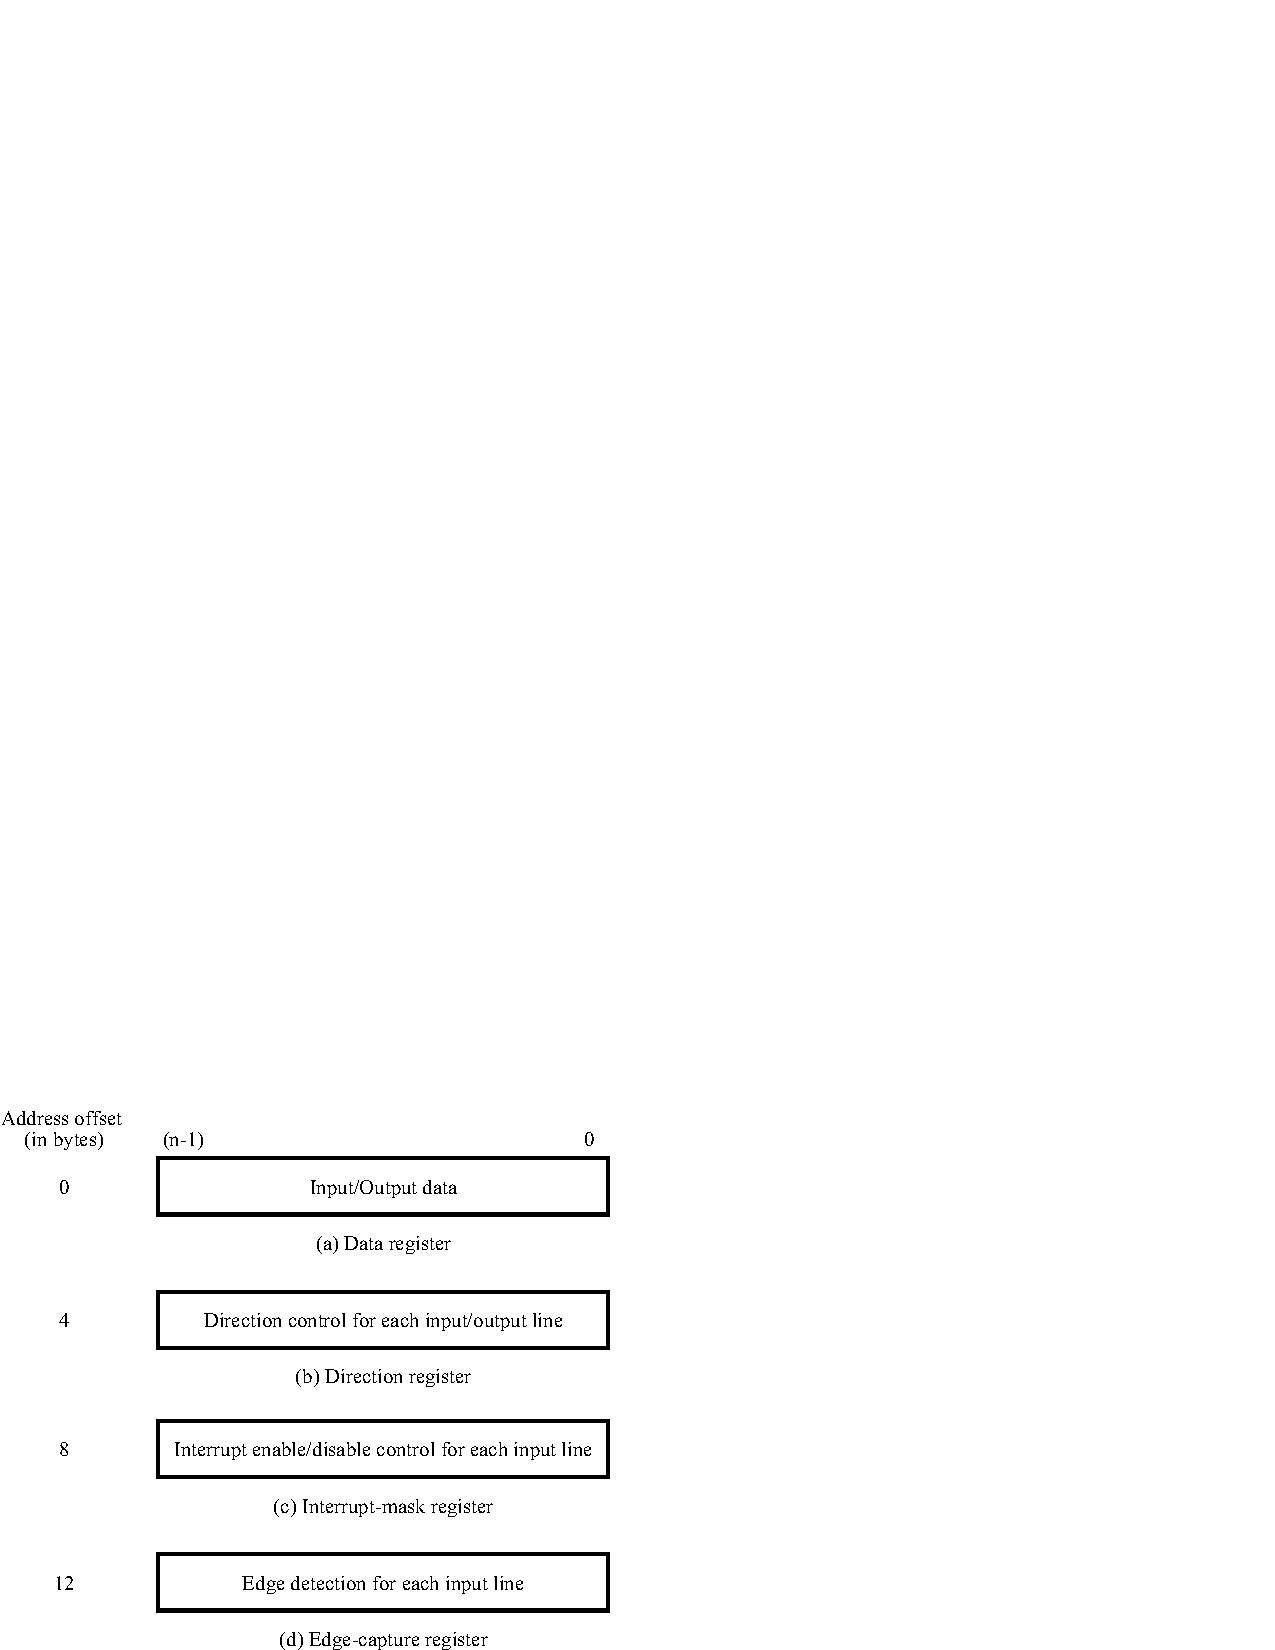
\includegraphics[scale=1]{figures/figureparallel.pdf}
	\end{center}
	\caption{Registers in the parallel port interface.}
\label{fig:parallel}
\end{figure}

\noindent
Each register is $n$ bits long. The registers have the following purpose:
\begin{itemize}
\item {\it Data} register: holds the $n$ bits of data that are transferred between the parallel 
port and the ARM processor. It can be implemented as an input, output, or a bidirectional register.
\item {\it Direction} register: defines the direction of transfer for each of the $n$
data bits when a bidirectional interface is generated.
\item {\it Interrupt-mask} register: used to enable interrupts from the
input lines connected to the parallel port.
\item {\it Edge-capture} register: indicates when a change of logic value is detected in 
the signals on the input lines connected to the parallel port. Once a bit in the edge
capture register becomes asserted, it will remain asserted. An edge-capture bit can be
de-asserted by writing to it using the ARM processor.
\end{itemize}
\noindent
Not all of these registers are present in some parallel ports. For example,
the {\it Direction} register is included only when a bidirectional interface is specified.
The {\it Interrupt-mask} and {\it Edge-capture} registers must be included if
interrupt-driven input/output is used.

~\\
The parallel port registers are memory mapped, starting at a specific {\it base} address.
This base address is the address of the {\it Data} 
register in the parallel port. The addresses of the other three registers have offsets 
of 4, 8, or 12 bytes (1, 2, or 3 words) from this base address. The DE10-Nano Computer has 
parallel ports connected to SW slide switches, KEY pushbuttons, and LEDs.

~\\
\noindent
{\bf Part I}
~\\
~\\
\noindent
Write an ARM assembly language program that displays a binary number on the green 
lights {\it LED}$_{3-0}$ on the DE10-Nano board. The other lights {\it LED}$_{7-4}$
should be off. 

~\\
\noindent
The parallel port in the DE10-Nano Computer connected to the green lights
{\it LED}$_{7-0}$ is memory mapped at the address {\sf 0xFF200000}. 
Figure~\ref{fig:LED} shows how the LEDs are connected to the parallel port bits.  

\begin{figure}[htb]
	\begin{center}
	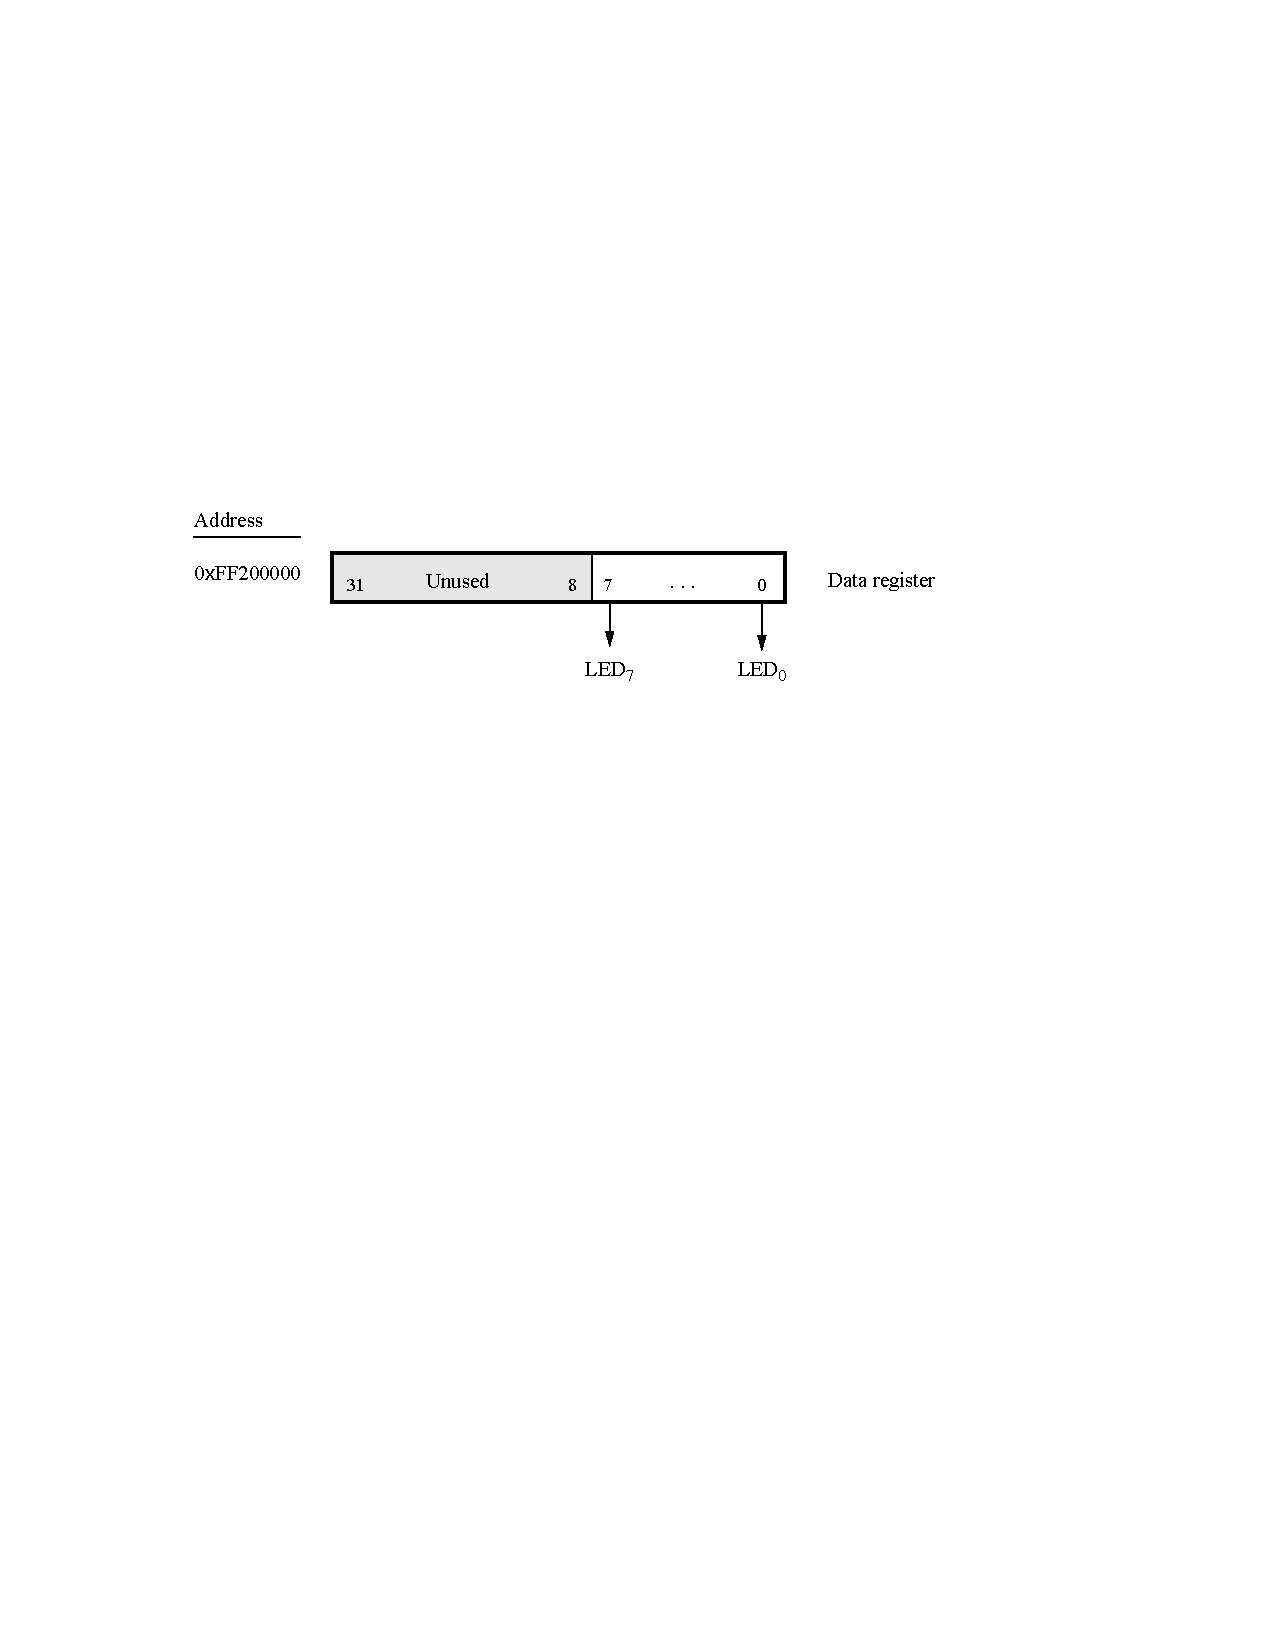
\includegraphics[scale=1]{figures/figureLED.pdf}
	\end{center}
	\caption{The parallel port connected to the green lights {\it LED}$_{7-0}$.}
\label{fig:LED}
\end{figure}

~\\
\noindent
Perform the following:

\begin{enumerate}
\item If {\it KEY}$_0$ is pressed on the board, you should set the number displayed on the
LEDs to 0. If {\it KEY}$_1$ is pressed and {\it SW}$_0$ is high, then increment the displayed
number to a maximum of 9. If {\it KEY}$_1$ is pressed and {\it SW}$_0$ is low, then decrement the
number to a minimum of 0. You can think of the displayed binary number as a {\it decimal digit},
since its value is restricted to be from 0 to 9 (\green{0000} to \green{1001}). The 
parallel port connected to the KEY pushbuttons has the base address
{\sf 0xFF200050}, as illustrated in Figure~\ref{fig:KEY}. The parallel port connected to
the SW slide switches has the base address {\sf 0xFF200040}, as illustrated in Figure~\ref{fig:SW}.
In your program, use polled I/O to read the {\it Data} registers of the {\it KEY} and {\it SW}
ports to check the status of the buttons and switches. When you are not pressing 
any {\it KEY} the {\it Data} register provides~0, and when you press {\it KEY}$_i$ the 
{\it Data} register provides the value 1 in bit position $i$. Once a button-press is detected,
be sure that your program waits until the button is released. You should not use the 
{\it Interruptmask} or {\it Edgecapture} registers for this part of the exercise.

\begin{figure}[htb]
	\begin{center}
	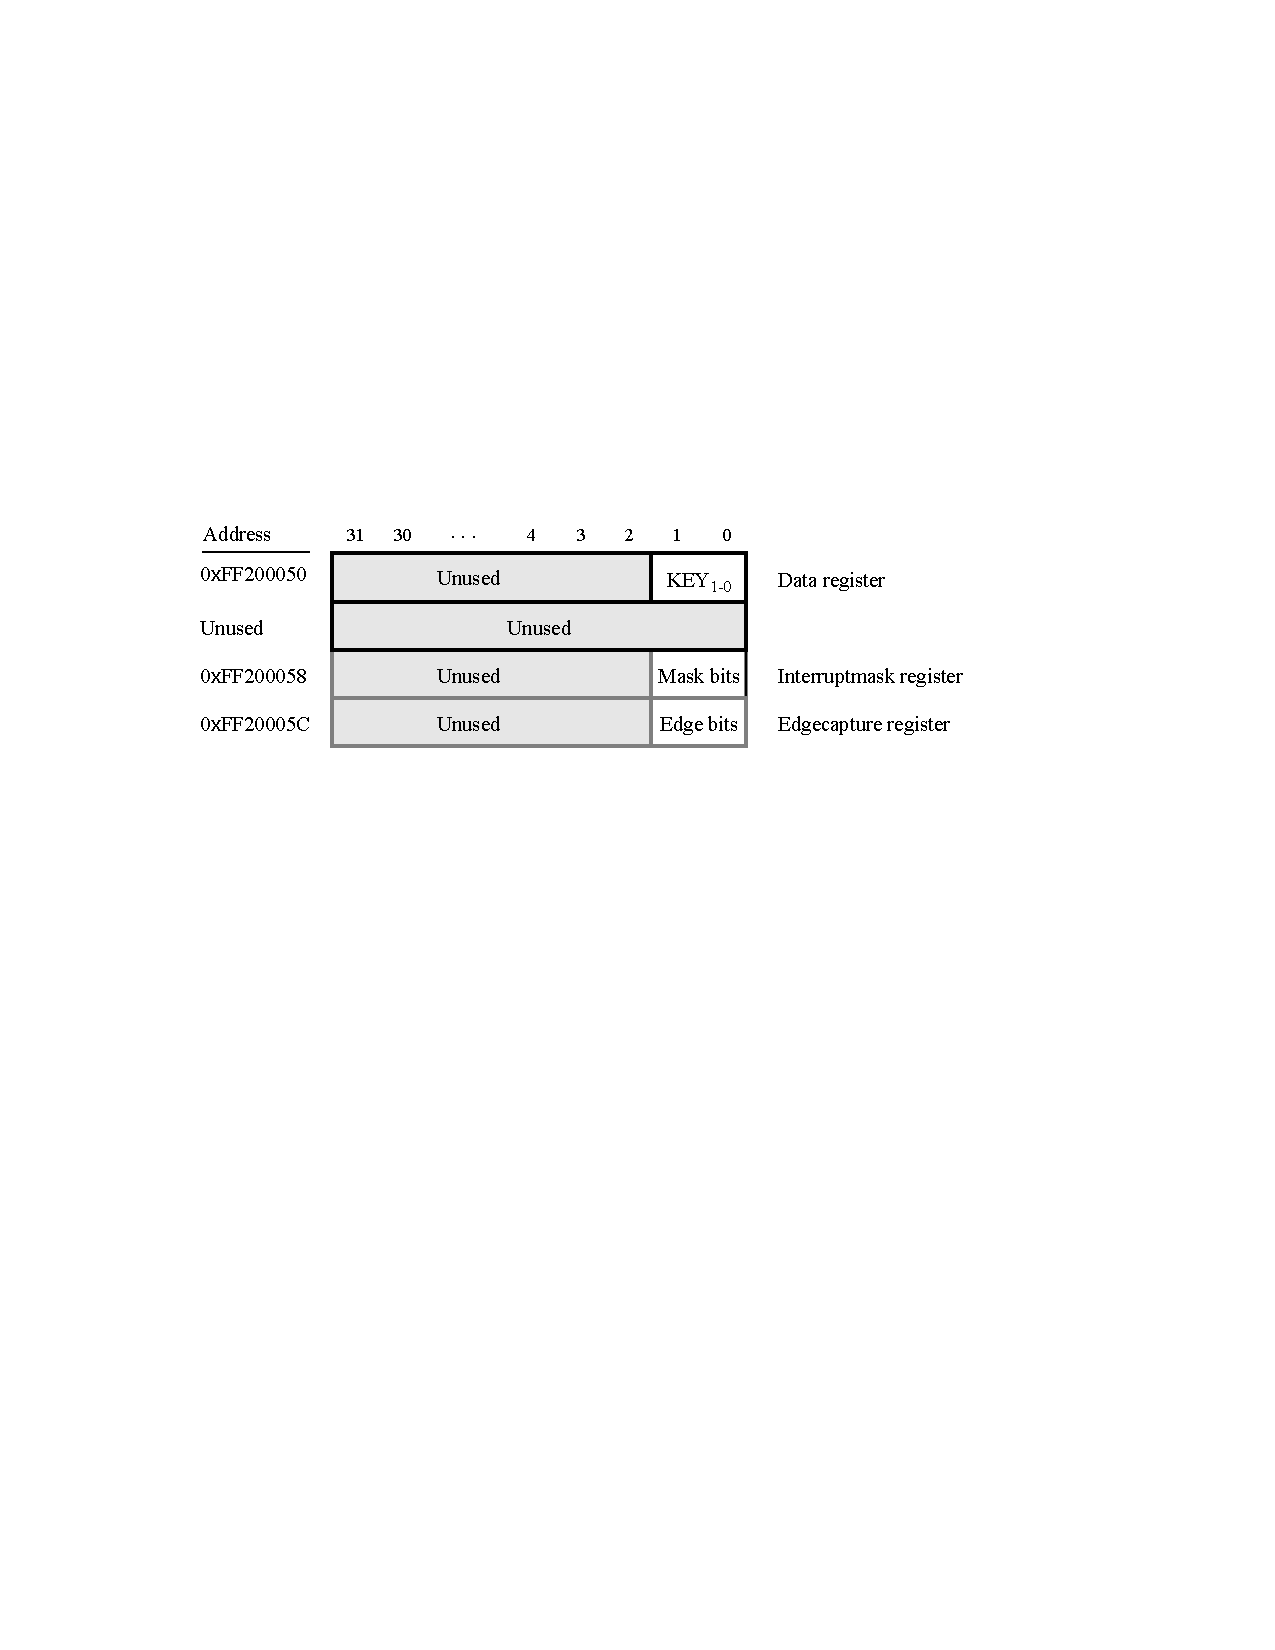
\includegraphics[scale=1]{figures/figureKEY.pdf}
	\end{center}
	\caption{The parallel port connected to the KEY pushbuttons.}
\label{fig:KEY}
\end{figure}

\begin{figure}[htb]
	\begin{center}
	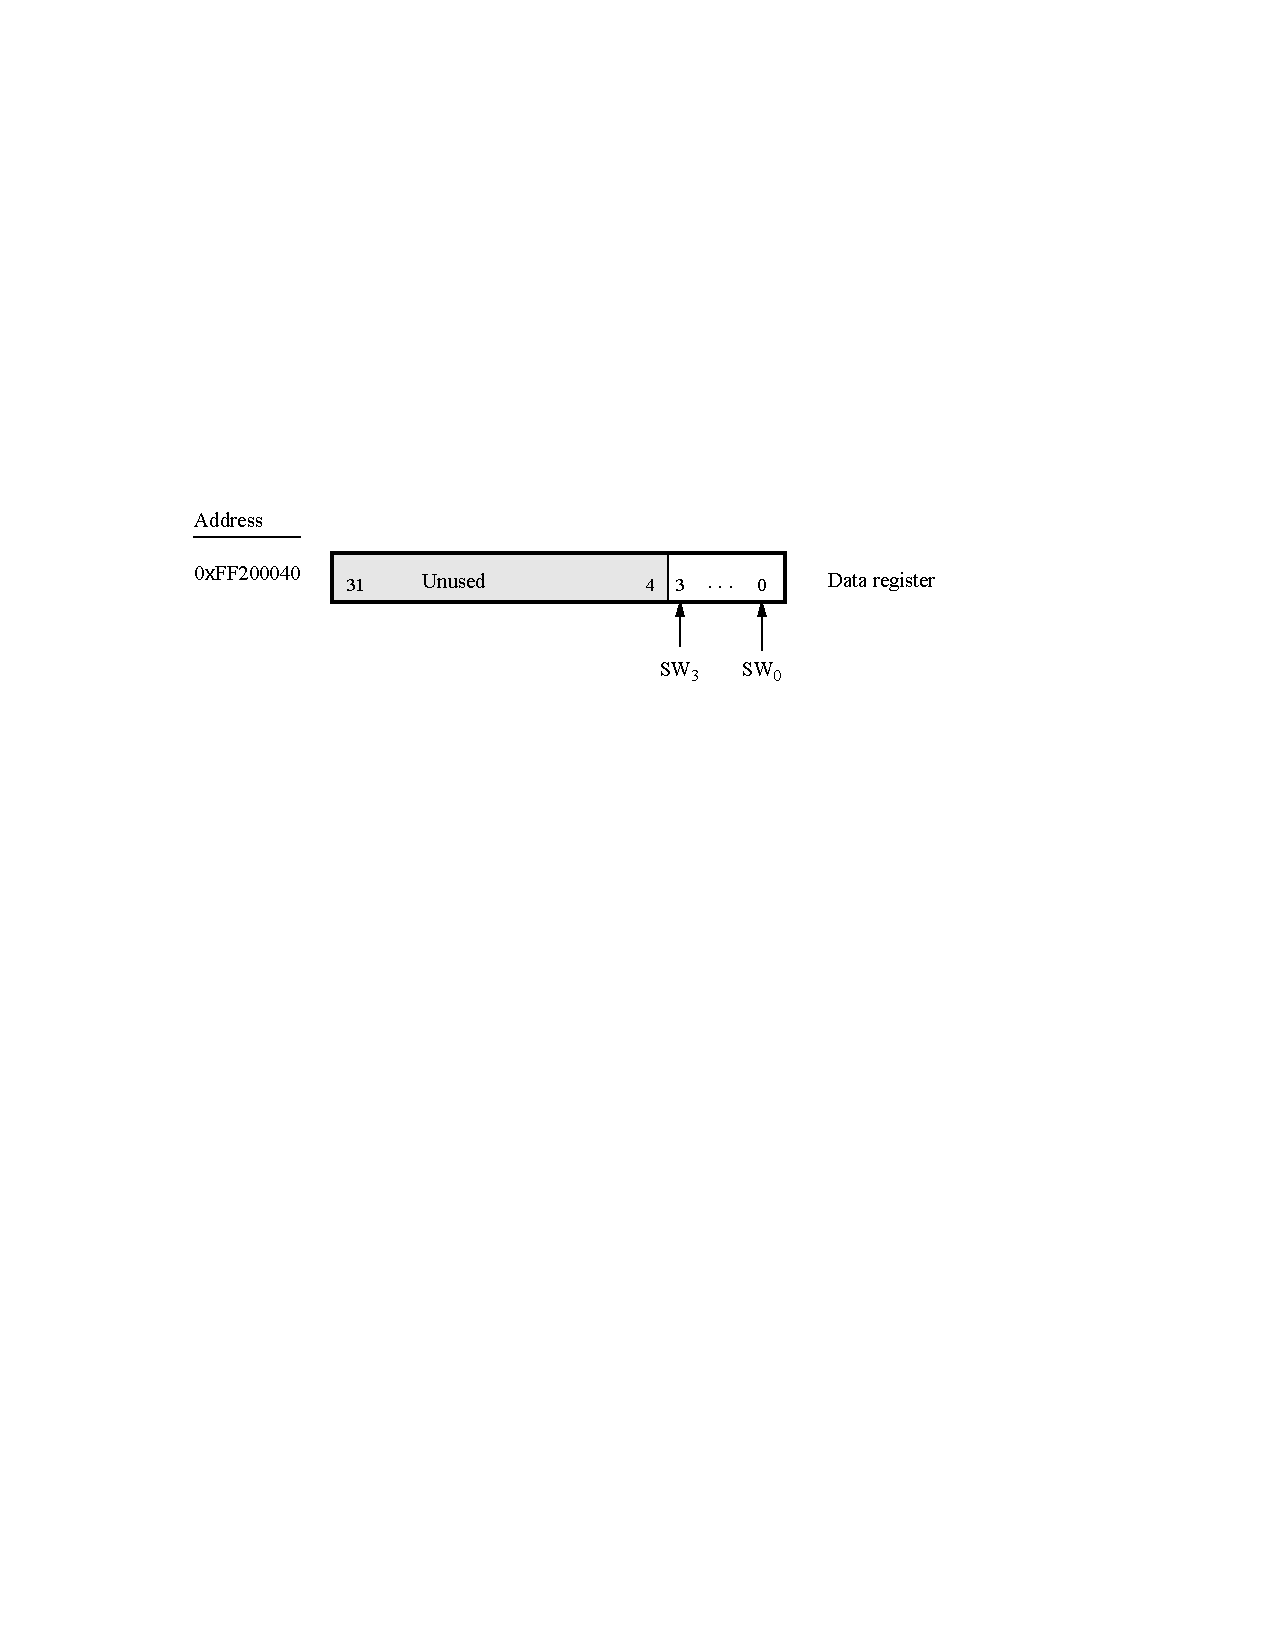
\includegraphics[scale=1]{figures/figureSW.pdf}
	\end{center}
	\caption{The parallel port connected to the SW slide switches.}
\label{fig:SW}
\end{figure}

\item Create a new folder to hold your solution for this part. Create a
file called {\it part1.s} and type your assembly language code into this file.

\item
Make a new Monitor Program project in the folder where you stored the {\it part1.s}
file. Use the DE10-Nano Computer for this project, and select ARM as the target
processor architecture.

\item
Compile, download, and test your program. 
\end{enumerate}

~\\
\noindent
{\bf Part II}
~\\
~\\
\noindent
In Part 1 you displayed a 4-bit binary number on the green LEDs. Since the value of the number was
restricted to be from 0 to 9, it could be considered as a {\it decimal digit}. For this part, 
you are to display {\it two} 4-bit binary values on the LEDs, representing {\it two} decimal digits:
the most-significant decimal digit should be shown on {\it LED}$_{7-4}$, and the least-significant
digit on {\it LED}$_{3-0}$. The decimal digits should function as a {\it counter} that takes
values from 00 to 99 (\green{00000000} to \green{10011001}). 
Write an ARM assembly language program that implements and displays
this counter. The counter should be incremented approximately every $0.25$ seconds. When the 
counter reaches the value 99, it should start again at 00. The counter should stop/start 
when {\it KEY}$_0$ or {\it KEY}$_1$ is pressed.

~\\
\noindent
To achieve a delay of approximately 0.25 seconds, use a delay-loop in your assembly language
code. A suitable example of such a loop is shown below.

\begin{minipage}[t]{12.5 cm}
\begin{lstlisting}[style=defaultArmStyle]
DO_DELAY: 	LDR		R7, =200000000 		// delay counter
SUB_LOOP: 	SUBS	R7, R7, #1
			BNE 	SUB_LOOP
\end{lstlisting}
\end{minipage}

~\\
\noindent
To avoid ``missing'' any button presses while the processor is executing the delay loop, you
should use the {\it Edgecapture} register in the {\it KEY} port, shown in Figure~\ref{fig:KEY}.
When a pushbutton is pressed, the corresponding bit in the {\it Edgecapture} register is
set to 1; it remains set until your program resets it to 0 by writing into the register.
~\\
~\\
\noindent
Perform the following:

\begin{enumerate}
\item Create a new folder to hold your solution for this part. Create a
file called {\it part2.s} and type your assembly language code into this file.

\item
Make a new Monitor Program project in the folder where you stored the {\it part2.s}
file. Use the DE10-Nano Computer for this project, and select ARM as the target
processor architecture.

\item
Compile, download, and test your program. 
\end{enumerate}

~\\
\noindent
{\bf Part III}
~\\
~\\
\noindent
In Part II you used a delay loop to cause the ARM processor to wait for approximately 0.25 
seconds. The processor loaded a large value into a register before the loop, and then 
decremented that value until it reached 0.  In this part you are to modify your code so that a
hardware timer is used to measure an exact delay of 0.25 seconds. You should use polled I/O to
cause the ARM processor to wait for the timer.

~\\
\noindent
The DE10-Nano Computer includes a number of hardware timers. For this exercise use the timer
called the ARM A9 {\it Private Timer}. As shown in Figure~\ref{fig:timer} this timer has 
four registers, starting at the base address {\sf 0xFFFEC600}. To use the timer you need
to write a suitable value into the {\it Load} register. Then, you need to set the enable
bit $E$ in the {\it Control} register to 1, to start the timer. The timer starts counting from
the initial value in the {\it Load} register and counts down to 0 at a frequency of 200 MHz. 
The counter will automatically reload the value in the {\it Load} register and continue counting 
if the $A$ bit in the {\it Control} register is set to 1.  When it reaches 0, the timer sets 
the $F$ bit in the {\it Interrupt status} register to 1.
You should poll this bit in your program to cause the ARM processor to wait for the timer. 
To reset the $F$ bit to 0 you have to write the value \texttt{1} into this bit-position. 

~\\
\begin{figure}[htb]
	\begin{center}
	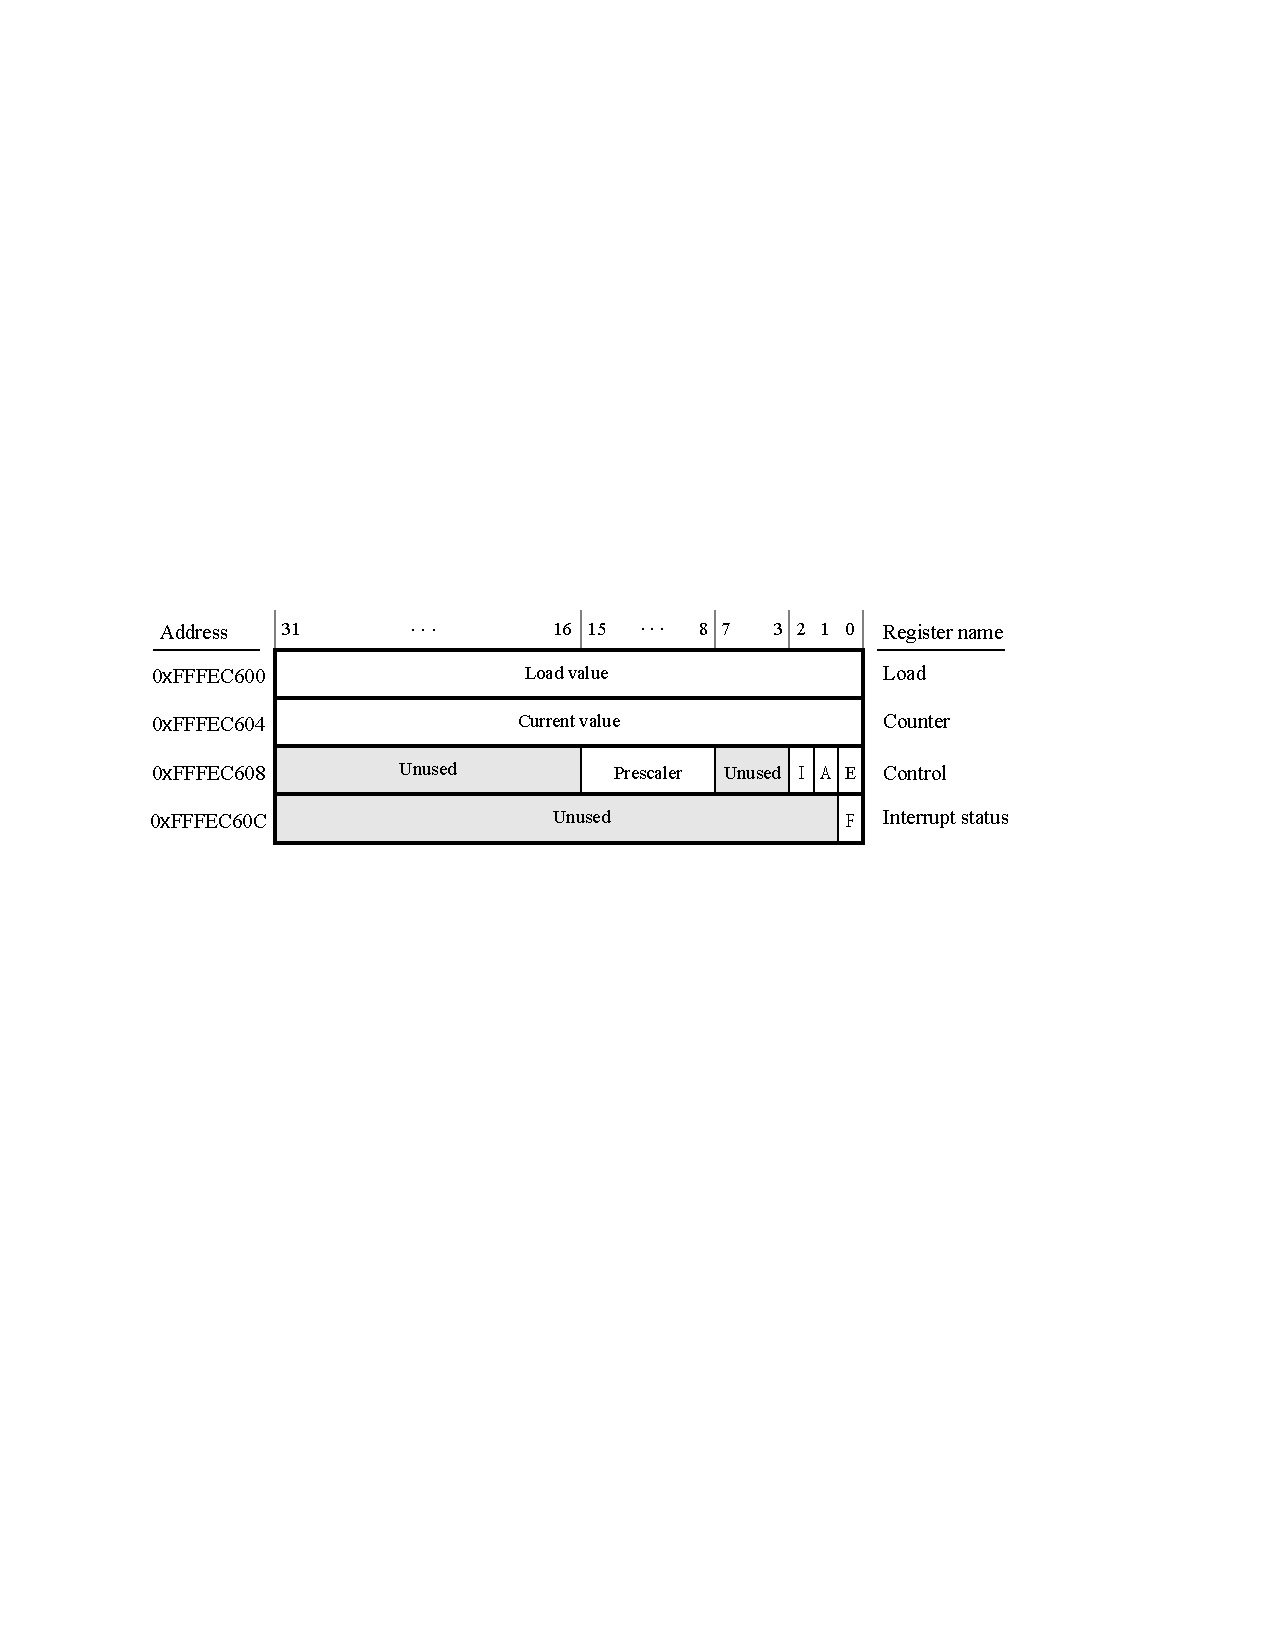
\includegraphics[scale=1]{figures/figuretimer.pdf}
	\end{center}
	\caption{The ARM A9 Private Timer registers.}
\label{fig:timer}
\end{figure}

~\\
\noindent
Perform the following:

\begin{enumerate}
\item Make a new folder to hold your solution for this part. Create a file called {\it part3.s} 
and type your assembly language code into this file.
\item Make a new Monitor Program project for this part of the exercise, and then compile, download, 
and test your program. 
\end{enumerate}

~\\
~\\
\noindent
{\bf Part IV}
~\\
~\\
\noindent
In this part you are to write an assembly language program that implements a real-time clock. 
Display the time on the Monitor Program's Terminal window in the format 
\blue{MM}:\blue{SS}, where \blue{\it MM} are minutes and \blue{\it SS} are seconds.
Measure time intervals of 1 second in your program by using polled I/O with the ARM A9 
Private Timer.  You should be able to stop/run the clock by pressing any KEY pushbutton.
When the clock reaches \blue{59}:\blue{99}, it should wrap around to \blue{00}:\blue{00}.

~\\
\noindent
Perform the following:

\begin{enumerate}
\item
Make a new folder for your solution to this part. Create a file called {\it part4.c} for 
your assembly language code. 
\item
Make a new Monitor Program project in the folder created for {\it part4.c}. In the screen 
shown in Figure~\ref{fig:terminal}, make sure to select {\sf JTAG\_UART\_for\_ARM\_0} as 
the {\it Terminal device}. Otherwise, no character output will appear on the Terminal window.
Refer to Exercise 2, Part IV, for information on using the JTAG* UART to communicate with 
the Monitor Program's Terminal window.  

\begin{figure}[htb]
	\begin{center}
	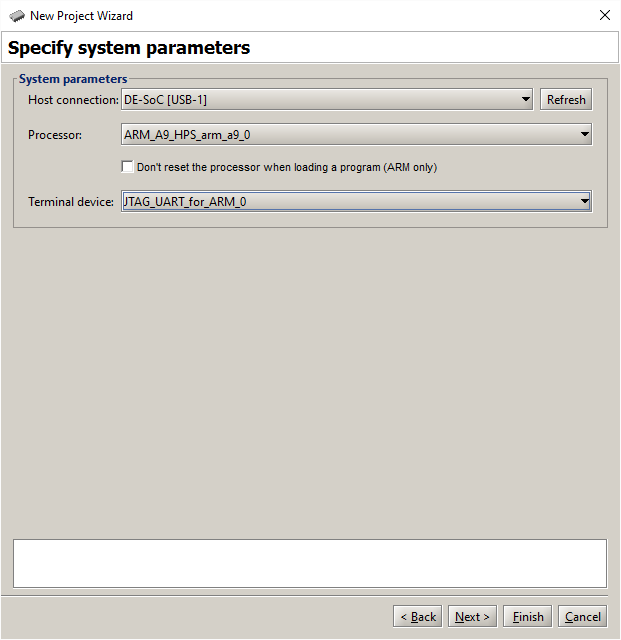
\includegraphics[scale=0.58]{figures/terminal.png}
	\end{center}
	\vspace{-0.25cm}\caption{Specifying the {\it Terminal device}.}
\label{fig:terminal}
\end{figure}

\item
You may wish to make use of the following text 
strings. The first one clears the Terminal window, and the second one returns the "cursor" to the 
upper-left corner of the window:
~\\
\begin{minipage}[t]{12.5 cm}
\begin{lstlisting}[style=defaultArmStyle]
CLR_SCRN: 	.asciz "\033[2J"
HOME: 		.asciz "\033[H"
\end{lstlisting}
\end{minipage}
\item
Test your program to see that it displays the real-time clock on the Terminal window, and that the
clock can be stopped/run by pressing the KEY pushbuttons.
\end{enumerate}


%%%%%%%%%%%%%%%%%%%%%%%%%%%%%%%%%%%%%%%%
%%% FPGAcademy Copyright Information %%%
%%%%%%%%%%%%%%%%%%%%%%%%%%%%%%%%%%%%%%%%

%Always put the copyright on a new page (clear page), with some vertical space from top
\clearpage
\vspace{1in}

\noindent

Copyright {\copyright} FPGAcademy.org. All rights reserved. FPGAcademy and the 
FPGAcademy logo are trademarks of FPGAcademy.org.  This document is provided 
"as is", without warranty of any kind, express or implied, including but not 
limited to the warranties of merchantability, fitness for a particular purpose 
and noninfringement. In no event shall the authors or copyright holders be 
liable for any claim, damages or other liability, whether in an action of 
contract, tort or otherwise, arising from, out of or in connection with the 
document or the use or other dealings in the document.
~\\
~\\
**Other names and brands may be claimed as the property of others.


\end{document}
